\documentclass{beamer}

\usepackage[latin1]{inputenc}
\usepackage{tikz}
\usetikzlibrary{arrows,shadows}

\usetheme{CambridgeUS}
\logo{
\includegraphics[scale=0.1]{redhat-logo.jpg}}
\title[OpenStack Liberty Keystone Midcycle ]{ Risk Assessment and Mitigation for Access Control mechanisms in OpenStack.
}
\author{Adam Young}
\institute{Red Hat Identity Management Team}
\date{Jul 15, 2015}
\begin{document}


\setbeamertemplate{navigation symbols}{}


\begin{frame}
  \titlepage
\end{frame}

\begin{frame}{Introduction}
  \begin{center}
    \begin{exampleblock}{}
      Risk Assessment and Mitigation for Access Control mechanisms in OpenStack.
    \end{exampleblock}
  \end{center}
\end{frame}

\begin{frame}
  \frametitle{Agenda}
  \tableofcontents
\end{frame}


\section{Threat Assessment}


\begin{frame}{Hypervisor Compromise: Tokens }
  \begin{itemize}
  \item validates the token
  \item Nova Compute Runs on the Hypervisor
  \item Tokens included included in requests
  \item Rogue VM Harvest Tokens
  \end{itemize}
\end{frame}


\begin{frame}{Hypervisor Compromise: Trusts}
  \begin{itemize}
  \item Allow for a long term delegation
  \item A rogue trust would by-pass the token expiry
  \item Without Trusts, passwords will be copied around, which is even worse.
  \item Easy to identify but you have to look
  \end{itemize}
\end{frame}


\begin{frame}{Authenticate via Token when fetching a token}
  \begin{itemize}
  \item Risk
      \begin{itemize}
        \item Any scope can be converted to another scope
        \item Expiration is not extended
      \end{itemize}
    \item Why:
      \begin{itemize}
      \item Web UI does not cache password
      \end{itemize}
    \item Mitigate
      \begin{itemize}
      \item Only allow unscoped to scoped transitions
      \item Requires a call to explicitly request a scoped token
      \end{itemize}
  \end{itemize}
\end{frame}

\section {Use of Tokens }

\begin{frame}{Why Are Tokens on Hypervisor}
  \begin{itemize}
  \item Boot and Teardown
    \begin{itemize}
    \item Barbican, Glance, Cinder, Neutron
    \end {itemize}
  \item Attach (Cinder)
  \item Periodic Refresh (Neutron)
  \item Snapshot (Glance)
  \end {itemize}
\end {frame}


\begin{frame}{Why Are Tokens on Hypervisor}
  \begin{block}{}
    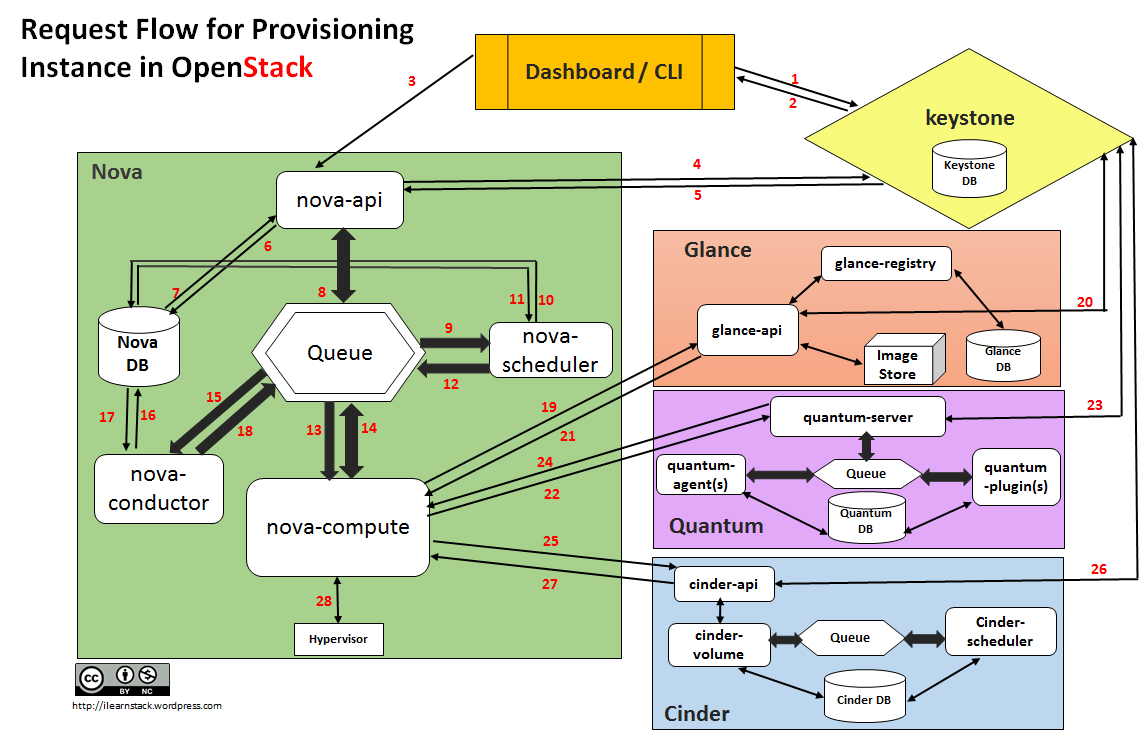
\includegraphics[scale=0.3]{request-flow1.png}
  \end{block}
  http://ilearnstack.com/2013/04/26/
\end {frame}


\begin{frame}{Big Tent Services that User Tokens}
  \begin{columns}[t,onlytextwidth]
    \begin{column}{.25\textwidth}
      \begin{itemize}
      \item Barbican
      \item Ceilometer
      \item Cinder
      \item Congress
      \item Cue
      \item Designate
      \end{itemize}
    \end{column}

    \begin{column}{.25\textwidth}
      \begin{itemize}
      \item Glance
      \item Heat
      \item Horizon
      \item Ironic
      \item Keystone
      \item Magneto DB
      \end{itemize}
    \end{column}

    \begin{column}{.25\textwidth}
      \begin{itemize}
      \item Magnum
      \item Manila
      \item Mistral
      \item Murano
      \item Neutron
      \item Nova
      \end{itemize}
    \end{column}

    \begin{column}{.25\textwidth}
      \begin{itemize}
      \item Sahara
      \item Search light
      \item Solum
      \item Swift
      \item TripleO
      \item Trove
      \item Zaqar
      \end{itemize}
    \end{column}

  \end{columns}

\end{frame}



\begin{frame}{Trove Uses Tokens}
  \begin{block}{}
    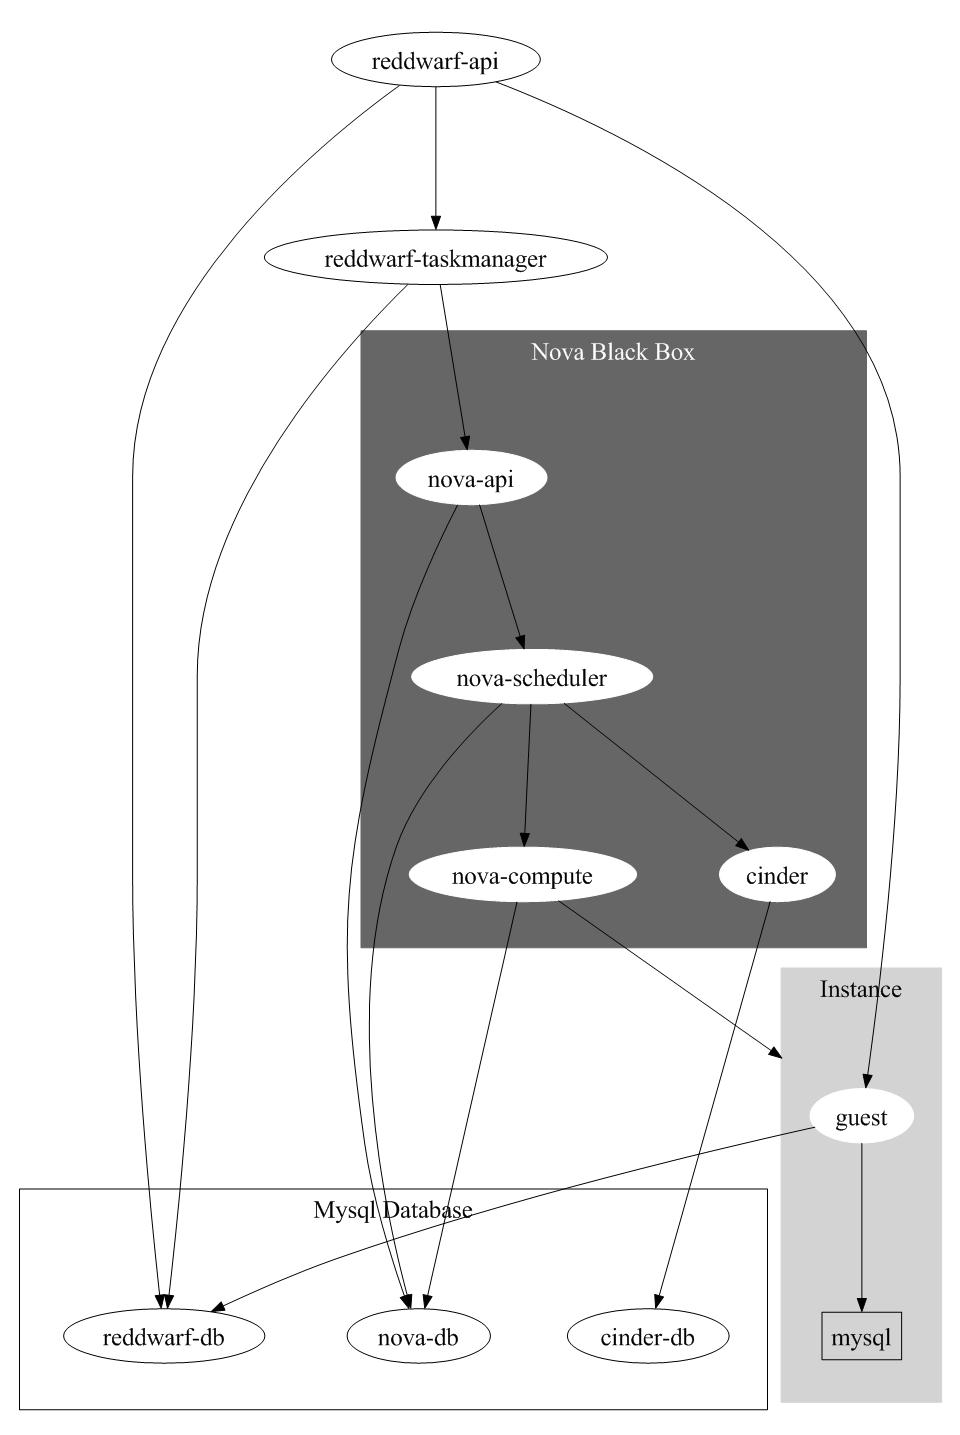
\includegraphics[scale=0.2]{Reddwarf-overview.jpeg}
  \end{block}
  https://wiki.openstack.org/wiki/Trove/trove-diagrams
\end {frame}

\begin{frame}{Sahara Uses}
  \begin{block}{}
    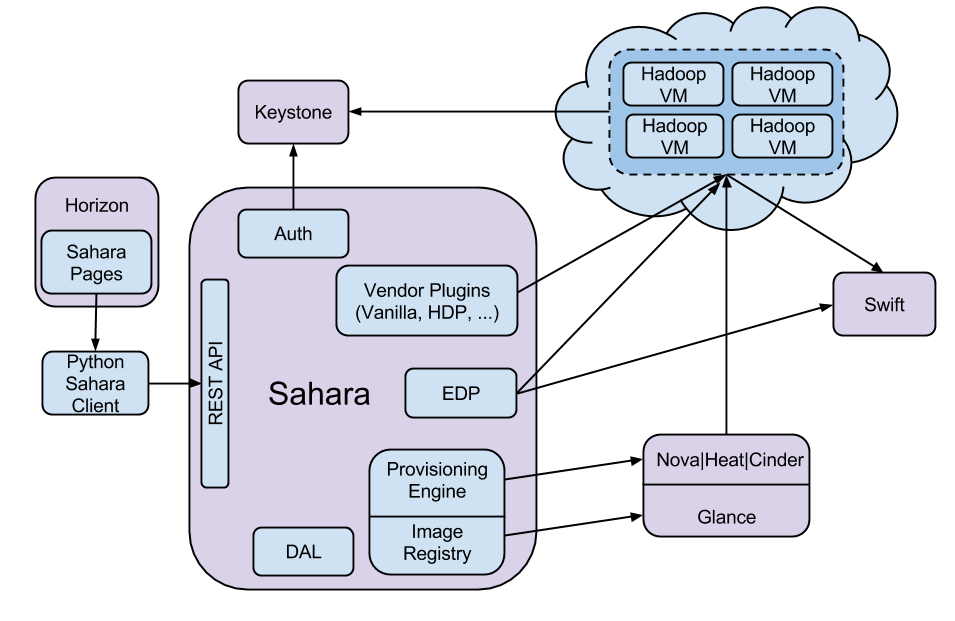
\includegraphics[scale=0.3]{sahara-architecture.png}
  \end{block}
  http://docs.openstack.org/developer/sahara/architecture.html
\end {frame}

\begin{frame}{Solum and Heat Use Tokens}
  \begin{block}{}
    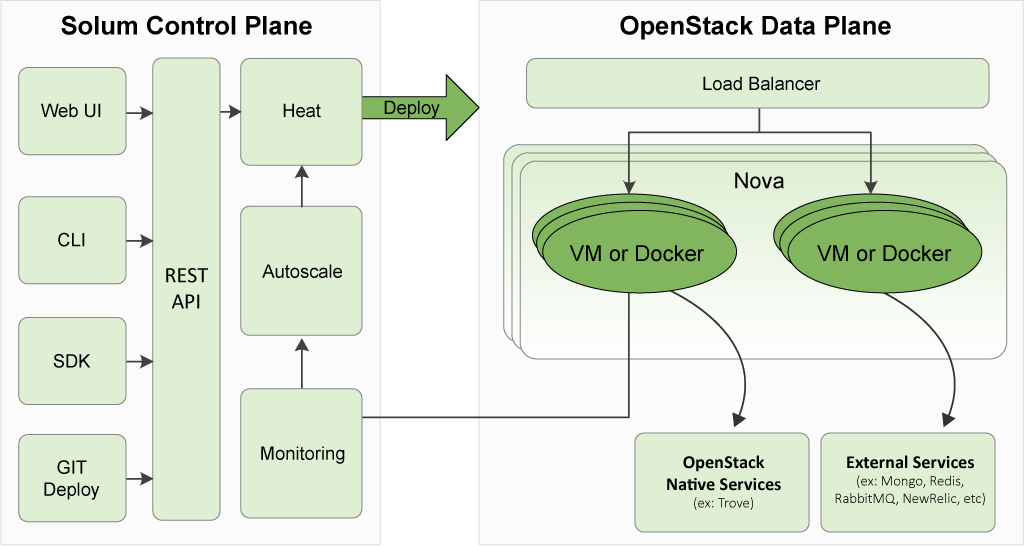
\includegraphics[scale=0.3]{solum-arch.png}
  \end{block}
  http://solum.io/img/chart.png
\end {frame}

\begin{frame}{Barbican Uses Tokens}
  \begin{block}{}
    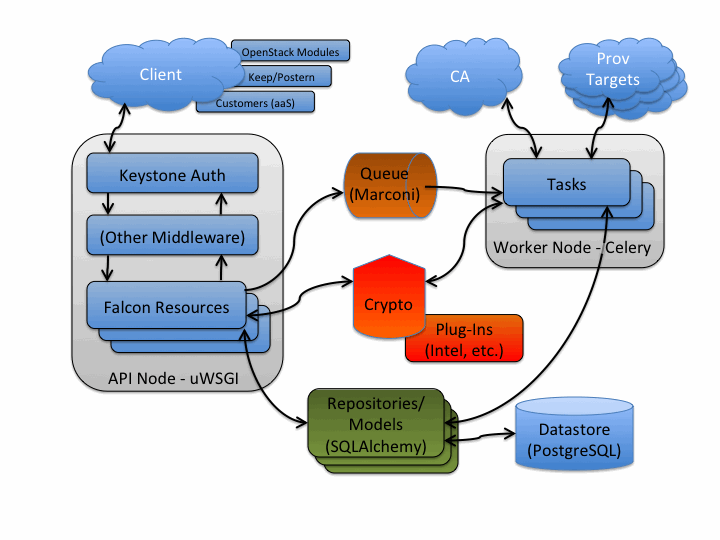
\includegraphics[scale=0.3]{barbican-arch.png}
  \end{block}
  https://github.com/cloudkeep/barbican/wiki/Architecture
\end {frame}



\section {Use Cases}

\begin{frame}{Scope of a Token}
  \begin{itemize}
  \item Most common role check is \textit{Admin} with no scope
  \item Most policy does not Check Roles
  \item  \textit{\_member\_ } role was added by Keystone to deal with migration from Tenant owning users
    \item A scoped token used on any service is valid for any \textit{\_member\_ } command anywhere else in the OpenStack Deployment
  \end{itemize}
\end{frame}


\begin{frame}{Member Use Cases}
  \begin{columns}[t,onlytextwidth]

    \begin{column}{.5\textwidth}
      \begin{itemize}
      \item Boot
        \begin{itemize}
        \item Heat
        \item Sahara
        \item Trove
        \end{itemize}
      \item Write Data
        \begin{itemize}
        \item Glance
        \item Trove
        \end{itemize}

      \end{itemize}
    \end{column}


    \begin{column}{.5\textwidth}
      \begin{itemize}
      \item Read Only
        \begin{itemize}
        \item Ceilometer
        \item Searchlight
        \end{itemize}

      \item Create Trust
        \begin{itemize}
        \item Heat
        \item Solum
        \end{itemize}
      \end{itemize}
    \end{column}
  \end{columns}
\end{frame}


\begin{frame}{Tenancy Administration Use Cases}
  \begin{columns}[t,onlytextwidth]

    \begin{column}{.5\textwidth}
      \begin{itemize}
      \item Nova
        \begin{itemize}
        \item Quotas
        \item Security Groups
        \item Key Pairs
        \end{itemize}
      \item Cinder
        \begin{itemize}
        \item Quotas
        \end{itemize}
      \item Glance
        \begin{itemize}
        \item images
        \end{itemize}
      \end{itemize}
    \end{column}

    \begin{column}{.5\textwidth}
      \begin{itemize}
      \item Keystone
        \begin{itemize}
        \item Assignments
        \end{itemize}

      \item Neutron
        \begin{itemize}
        \item Networks
        \item Subnets
        \item Extensions
        \end{itemize}
      \end{itemize}
    \end{column}
  \end{columns}
\end{frame}


\begin{frame}{Service Administration Use Cases}
  \begin{columns}[t,onlytextwidth]

    \begin{column}{.5\textwidth}
      \begin{itemize}
      \item Nova
        \begin{itemize}
        \item Hypervisors
        \item Floating ip associate
        \item Cells
        \end{itemize}
      \end{itemize}
    \end{column}

    \begin{column}{.5\textwidth}
      \begin{itemize}
      \item Keystone
        \begin{itemize}
        \item Roles
        \item Service Catalog 
        \item Policy
        \end{itemize}
      \end{itemize}
    \end{column}
  \end{columns}
\end{frame}


\section {Design Considerations}

\begin{frame}{Constraints}
  \begin{itemize}
  \item  Deployments expect the current stock policy files to work
  \item Global Admin to the rescue
  \item Where is the scope?
  \end{itemize}
\end{frame}


\begin{frame}{Role vs Scope}
  \begin{itemize}
  \item Matching Scope should not be customized
    \begin{itemize}
    \item  Engineering decision
    \item  based on the object structure
    \end{itemize}
  \item Role Assigned to API should be customizable
    \begin{itemize}
    \item Chose the roles appropriate to the organization
    \item Default to \textit{Admin} if not specified for target
    \end{itemize}
  \end{itemize}
\end{frame}
  

\begin{frame}{Global Admin}
  \begin{itemize}
  \item Most stock policy files have an account to fix things
   \begin{itemize}
    \item Chose the roles appropriate to the organization
    \item Default to \textit{Admin} if not specified for target
    \end{itemize}
  \end{itemize}
\end{frame}
  

\begin{frame}{Global Admin}
  \begin{itemize}
  \item Most stock policy files have an account to fix things
    \begin{itemize}
    \item Nova has it in code: nova/tree/nova/policy.py
    \item return creds['is\_admin'] == self.expected
    \item "os\_compute\_api:os-lock-server:unlock:unlock\_override": "rule:admin\_api",
    \item "admin\_api": "is\_admin:True",
    \end {itemize}
  \item Keystone has  ADMIN\_TOKEN/OS\_SERVICE\_TOKEN
  \item Check Role:admin without checking Scope
  \end{itemize}
\end{frame}



\begin{frame}{Where is the Scope}
  \begin{itemize}

  \item project\_id in the URL
    \begin{itemize}
    \item Nova list servers
    \item http://hostname:8774/v2/<project\_id>/servers/detail
    \item Trove list databases for instance
    \item https://hostname/v1.0/<project\_id>/instances/<instance\_id>/databases
    \item Keystone grant role to user on project
    \item PUT http://hostname:35357/projects/<project\_id>/users/<user\_id>/roles/<role\_id>
    \item must confirm with database record
    \end{itemize}

  \item Use the scope from the token
    \begin{itemize}
    \item Glance image list
    \item http://hostname/v1/images
    \item Won't work with a global admin
    \end{itemize}
  \end{itemize}
\end{frame}

\begin{frame}{Where is the Scope (Continued)}
  \begin{itemize}

    
  \item Fetch object from Database
    \begin{itemize}
    \item Ceilometer Rules mostly have
    \item "context\_is\_project": "project\_id:%(target.project\_id)s"
    \item Keystone add user to group (Domain scoped)
    \item PUT /groups/<group\_id>/users/<user\_id>
    \end{itemize}

  \item Object is not scoped to a project
    \begin{itemize}
    \item Keystone User owns Credentials and Trusts
    \item Domains own projects
    \item Barbican user owns secrets
    \end{itemize}
  \end{itemize}
\end{frame}


\begin{frame}Neutron Policy Rules{}
  \begin{itemize}
  \item "shared\_*":
    \begin{itemize}
    \item "field:networks:shared=True",
    \item "field:firewalls:shared=True",
    \item "field:firewall\_policies:shared=True",
    \item "field:subnetpools:shared=True",
    \item "field:address\_scopes:shared=True",
    \end{itemize}
  \item "get\_subnetpool":
    \begin{itemize}
    \item "rule:admin\_or\_owner or rule:shared\_subnetpools",
    \end{itemize}
  \item (unscoped) admin role check OR access to the API is global
  \item Limited to read only.
  \end{itemize}
\end{frame}

\begin{frame}What is a Role?{}
  \begin{itemize}
    \item A label for a set of permissions across multiple services
    \item But we have no way to share role information between services or endpoints with stock policy files
  \end{itemize}
\end{frame}

\begin{frame}{Problems with Role Assignments today}
  \begin{itemize}
  \item If I can assign one role, I can assign any role
  \item Admin role is not scoped to a proejct
  \item If I can assign admin, I am admin
  \item Need to restrict ability to assignment only the roles/scope a user has assigned to them.
  \end{itemize}
\end{frame}


\section {Dynamic Policy}


\begin{frame}{Original Dynamic Policy Design}
  \begin{itemize}
  \item Graduate oslo policy to a library
  \item Common code to enforce policy on a token
  \item Fetch policy from Keystone
  \item Provide a unified policy file
  \item Database schema to hold policy rules.  
  \item Hierarchical roles
  \item Generate rules from hierarchical roles
  \item Break member up into smaller roles.
  \item Use the smaller roles in the Policy targets.
  \item Users can only assign a role that they themselves have on the designated scope.
  \end{itemize}
\end{frame}

\begin{frame}{Dynamic Policy Successes}
  \begin{itemize}
  \item Graduate oslo policy to a library complete
  \item Fetch policy from Keystone no targeted at URLs, not Endpoint Ids
  \item Kent has Proof of Concept for Database
  \end{itemize}
\end{frame}


\begin{frame}{Dynamic Policy Adjustments}
  \begin{itemize}
  \item Unified Policy File may conflict dynamic natures of microversions
  \item Hierarchical Roles now includes role namespacing
  \item Kent design is better for querying
  \end{itemize}
\end{frame}


\subsection {Policy Distribution}


\begin{frame}{Why not Use Configuration Management System}
  \begin{itemize}
  \item Can be done, but has drawbacks
  \item Removes Keystone's ability to determine which policy file to fetch
  \item Most installations treat Policy as static, and will not update even if Keystone updates
  \item Extracts Policy out of the application management flow
  \item In the future, project specifc policy will require futher integration
  \end{itemize}
\end{frame}


\begin{frame}{Why fetch by URLs}
  \begin{itemize}
  \item May not get a unified policy file
  \item Need to server separate policy for each service
  \item If customized for a specific server, we need to serve the policy for that server
  \item While this might be multiple \textit{endpoints}we can treat all endpoints with the same URL as one endpoint for policy reasons
  \item CMS can calculate the URL prior to registering endpoint
  \item With endpoint\_id: register, retreive ID, inject into config, restart server
  \item For most cases, middelware could deduce the URL from a request.
  \item Why not Free form label?
    \begin{itemize}
    \item Might be useful in the future
    \item Would still require mapping to the endpoint 
    \end{itemize}
  \end{itemize}
\end{frame}


\begin{frame}{Where do we fetch?}
  \begin{itemize}
  \item Oslo.policy is not specific to RBAC
  \item Fetching from Keystone is not specific to Oslo.policy
  \item After token validation
  \item Before Policy is called
  \item Using Policy for Endpoint binding in Middleware
  \end{itemize}
\end{frame}


\begin{frame}{auth\_token vs policy middleware}
  \begin{itemize}
  \item auth\_token is purely a convenience, 
  \item does not require modifying pipelines
  \item Separate middleware would be cleaner
  \item Compromise: auth\_token as a series of separateable middleware modules
  \end{itemize}
\end{frame}

\begin{frame}{Enforce policy from middleware}
  \begin{itemize}
  \item enforce policy on URLs, not random strings inside the code
  \item role/scope split
    \begin{itemize}
    \item only the role portion
    \item this makes the most sense for customization
    \end{itemize}
  \item Scope would have to be enforced after database fetch for many resources
  \item Middleware can return HTTP 401 with extra knowledge of what role is required
    \begin{itemize}
    \item Bends the standard, but does not break it
    \end{itemize}
  \end{itemize}
\end{frame}


\begin{frame}{Single Unified Policy File}
  
  \begin{itemize}
  \item  \textbf{Not stock policy}
    \begin{itemize}
    \item Kept in its own repo
    \item only deployed deliberately
    \end {itemize}
  \item Common section for common rules
  \item Specify lowest role necessary
  \item Single Policy Header
  \item Move toward a single File
  \item Hierarchical Roles
  \item Break member up into smaller roles
  \item Change the rules for specific API policy enforcement points to know about the new roles.
  \end{itemize}
\end{frame}


\subsection {Roles}


\begin{frame}{Implied Roles}
  \begin{itemize}
  \item Hierarchical is overloaded term but what NIST uses
  \item Implied roles:
    \begin{itemize}
    \item Explicit-role IMPLIES Implicit-Role
    \item Impicit Roles can IMPLY other Implicit-Roles
    \item Admin IMPLIES Member
    \item Member IMPLIES both Read-Only and Writeable
    \end{itemize}
  \item A user is assigned a role at the top of the hierarchy
  \item A target specifies a role as low on the hierarchy as possible
  \item A user can then delegate an implicit role instead of explicit
  \end{itemize}
\end{frame}


\begin{frame}{Global Admin}
  \begin{itemize}
  \item   Better Global Admin
    \begin{itemize}
    \item Global admin means user is in admin role on admin domain
    \item In order to test that outside of Keystone server, we need to be able to query Keystone config remotely
      Added Benefit: allows a way to query default domain as well
    \end{itemize}
  \item Alternative to Global Admin
    \begin{itemize}
    \item Provide a means for a specific user to get a token scoped to any project with any role
    \item Is it really any worse?
    \end{itemize}
  \end{itemize}
\end{frame}


\begin{frame}{Role Namespaces}
  \begin{itemize}
  \item Roles are lables.
  \item Currently, all roles are global
  \item Roles hould map to the services
    \begin{itemize}
    \item \textit{Admin} versus \textit{Compute.admin, network.admin}
    \end{itemize}
  \item Implied roles can still work across namespaces
    \begin{itemize}
    \item Compute.boot implies network.reader
    \end{itemize}
  \item Can expand the role of Keystone beyond Undercloud:
    \begin{itemize}
    \item \textit{Wordpress.editor}
    \item \textit{Gerrit.approver}  implies \textit{Git.committer}
    \end{itemize}
  \item Segregated by Project Scope as well
    \begin{itemize}
    \item \textit{Gerrit.approver} on \textit{Openstack/Keystone} vs
    \item \textit{Gerrit.approver} on \textit{Openstack/Nova}
    \end{itemize}
  \end{itemize}
\end{frame}


\begin{frame}{Scope All Entities}
  \begin{itemize}
  \item Keystone Service level entities be owned by the Admin Domain
    \begin{itemize}
    \item Services
    \item Endpoint
    \item Regions
    \item Roles
    \end{itemize}
  \item Lends itself to better delegation in the future
    \begin{itemize}
    \item Scope Roles under services to Namespace
    \end{itemize}
  \end{itemize}
\end{frame}





\begin{frame}{How Do We Know What Permissions to Delegate?}
  \begin{itemize}
  \item Changes are rare enough that we can figure out statically
  \item When doing a Nova Boot, the Nova client can be smart enough to get the right token.
  \item All those things that call Nova boot need to be smart enought, too
  \item As things get more complicated, we can run Tempest against policy in permissive mode and see what would have gotten rejected.
    \begin{itemize}
    \item This approach works for SELinux and AppArmor
    \end{itemize}
  \end{itemize}
\end{frame}

\begin{frame}{Requesting a Token with a subset 	of roles}
  \begin{itemize}
  \item Request only the role required for the task at hand
  \item ``I need a token for booting a VM''
  \item Ideally, a token would have only a single role
    \begin{itemize}
    \item Added Benefit: Fernet-style token implementations smaller
    \end{itemize}
  \end{itemize}
\end{frame}


\begin{frame}{Long lived delegations}
  \begin{itemize}
  \item shorter the token lifespan  = smaller attack surface
  \item No risk of timing out on long uploads etc
  \item Nova could request a read only token for other services during boot.
  \item Trusts and OAUTH1 should use the same logic
    \begin{itemize}
    \item OAUTH Consumer becomes user in a custom domain
    \end{itemize}
  \end{itemize}
\end{frame}


\begin{frame}{Unified Delegation}
  \begin{itemize}
  \item Role assignment Follows Trust model except we add concept of \textit{Position} or permanent role assignment
    \begin{itemize}
    \item A user is assigned to a \textit{position}
    \item All permanent role assigments happen from \textit{position} to \textit{position}
    \item A user can only delegate to a \textit{position} a role that they themself are assigned,either explicitly or implicitly
    \item If a \textit{position} goes unfilled, role assignments previously made from that \textit{position} are:
      \begin{itemize}
      \item inactive until it is filled again, or
      \item are approved by a higher authority
      \end{itemize}
    \end{itemize}
  \end{itemize}
\end{frame}

    

\begin{frame}{Task Ordering}
  \begin{itemize}
  \item Each commit should show value stand alone
  \item Front load the changes that must be approved by the other projects
  \item Start with dynamic fetch, manual management
  \item Continue to refine the plan
  \end{itemize}
\end{frame}



\begin{frame}{Questions}
  \begin{center}
    \begin{exampleblock}{}
      Questions?
    \end{exampleblock}
  \end{center}
\end{frame}

\end{document}
